\section{Genetic Programming}
In the second part of the project, we had to find Newton's law of universal
gravitation using genetic programming.

\subsection{Fitness Measurement}
Our original plan was to sample the Earth's trajectory only once with the
target law, that is to say Newton's law of universal gravitation. Then to
compute the Earth's trajectory for each new individual (i.e. for each new law)
produced by the genetic algorithm. The fitness score of each individual would
have been the sum of the distances between two corresponding points in the
samplings as explained in Figure \ref{error_1}. However, EASEA does not allow
the
user to call the generated function with
"dynamic" arguments, so it was not possible to perform the sampling anew. So we
had to abandon this idea.\\

After some thought, we decided to do only one sampling with the correct
universal law of gravitation. Knowing the position of the Earth in the
heliocentric referential, we were able to compute the norm of the attractive
force existing between Earth and Sun. Instead of computing the sum of the
errors between the coordinates like in Section \ref{evol}, the error was set to
correspond to the average of the differences between the real force and the
estimated force at each point of the path (\Figure \ref{error_2}).\\

\begin{figure}
    \[ error = \frac{1}{n} \sum_{i=0}^{n} | f(p_{i}) - \hat{f}(p_{i}) | \]
    where:
    \begin{itemize}
        \item \(n\) denotes the number of samples (typically 1024)
        \item \(p_{i}\) corresponds to the i-th sampled point on the real
              Earth's
              trajectory
        \item \(f\) correspond to Newton's law of universal gravitation
        \item \(\hat{f}\) is the estimation of the Newton's law of universal
              gravitation made by the program
    \end{itemize}
    \caption{Expression of the error for evolutionary algorithms}
    \label{error_2}
\end{figure}

Although this approach worked (as shown in Section \ref{gp}), it
has a major flaw with compared to our first idea. We need the force at each
point to find
the target law. In other words: we need to know something that is only
computable with the
real law in order to find the law...\\

\subsection{Newton's law of universal gravitation}
\label{gp}
In order to find Newton's law of universal gravitation using genetic
programming we needed to adjust some parameters on top of the fitness
measure.\\

The first thing to adjust was the mass of the planets. As far as we know, EASEA
is limited to float for genetic programming so pursuing any computation with
involving the Sun's mass is quite challenging. In our first attempt, we
immediately got overflaws. Once again, we had to backtrack and experiment with
other planets with a smaller mass. We settled for Earth and Moon that both have
a significantly lower mass.\\

Initially, we gave our individual four binary operators (+,-,*,/), three
constants (the mass of the sun, the mass of the earth and the gravitational
constant) and
one variable (the distance between the two heavenly bodies). The program also
had the possibility to generate constants between zero and one.\\

Figure \ref{gp_1} shows it is possible to find the law albeit at the expense of
a long computation time. In fact in order to find the exact law we needed to
create a large population (typically 5000 individuals) and let the algorithm
works during hundreds of generations (in this instance 500 generations).\\

It is also worth mentionning that the algorithm did not always converged to the
correct law but sometimes to laws that look really different. Some of them gave close results (Figure
\ref{gp_2}) but other outputed irrelevant trajectories (Figure
\ref{gp_3}). The latter being explained by stopping the evolution of too few individuals too early.\\

When used with a wide enough population genetic programming is an impressively efficient method capable of finding complex equations like Newton's law of universal gravitation.\\

\begin{figure}
    \begin{lstlisting}
495        294.404s         2480000         2480000 0.000000000e+00 1.6e+12 2.1e+13 3.1e+14
496        295.234s         2485000         2485000 0.000000000e+00 9.9e+11 1.7e+13 3.1e+14
497        296.091s         2490000         2490000 0.000000000e+00 1.7e+12 2.1e+13 3.3e+14
498        296.890s         2495000         2495000 0.000000000e+00 1.6e+12 2.0e+13 3.1e+14
499        297.673s         2500000         2500000 0.000000000e+00 1.5e+12 2.0e+13 3.1e+14
EASEA LOG [INFO]: Seed: 1676057640
EASEA LOG [INFO]: Best fitness: 0
EASEA LOG [INFO]: Elapsed time: 297.674
(((s)*((e)*(G)))/((r)*(r)))
\end{lstlisting}
    \caption{Output of the EASEA genetic program (500 generations of 5000
        individuals)}
    \label{gp_1}
\end{figure}

\begin{figure}
    \center
    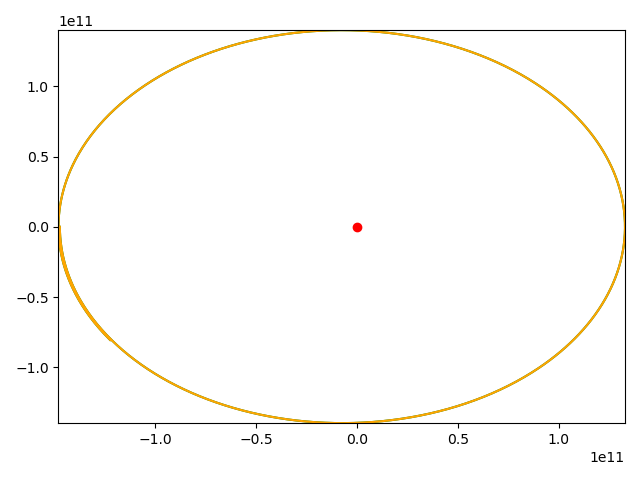
\includegraphics[scale=.3]{img/newton_gp_1.png}
    \caption{Earth trajectory with the result of a genetic program (\(f(r) = G \left( \frac{M_{Sun}(G + M_{Moon})}{r^2} + 0.95 \right)\))}
    \label{gp_2}
\end{figure}

\begin{figure}
    \center
    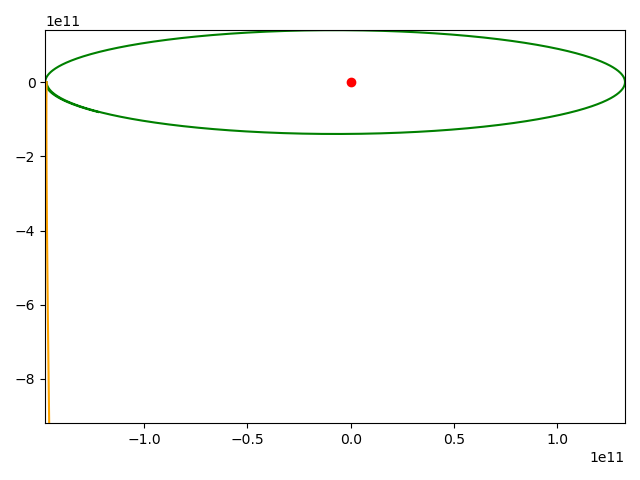
\includegraphics[scale=.3]{img/newton_gp_2.png}
    \caption{Earth trajectory with the result of a genetic program (\(f(r) = ((((\frac{M_{Earth}}{0.460538}/0.460538)/0.460538)/r)+(((\frac{M_{Earth}}{0.460538})/0.392773)/(r-G))+(((G-r)-(r+r))+(\frac{M_{Earth}}{0.460538})/(r-G)))))\))}
    \label{gp_3}
\end{figure}